\chapter*{Appendices}
% \label{ch:appendices}
%this relabels the table of contents to have Figure A1 instead of Figure 7.1
\setcounter{figure}{0}
\setcounter{equation}{0}
\setcounter{table}{0}
\renewcommand{\thefigure}{A\arabic{figure}}
\renewcommand{\theequation}{A\arabic{equation}}
\renewcommand{\thetable}{A\arabic{table}}
\addcontentsline{toc}{chapter}{Appendices}


\newpage
\section*{Appendix A: Supplementary Information for Chapter 3}
\addcontentsline{toc}{section}{Appendix A: Supplementary Information for Chapter 3}
\subsection*{Atmospheric loading correction}
Variable atmospheric pressure can cause cm-scale crustal deformation \cite[]{magie1969source,darwin1882xlvi,petrov2004study} and has been detected in GPS time series \cite[]{vandam1994atmospheric,dong2002anatomy}.  Atmospheric contributions therefore need to be removed from the GPS time series in order to isolate the ice load effects.  To correct for air pressure loading, we use pre-computed Atmospheric Loading Displacements (ALD) provided by the Atmospheric Pressure Loading Service (http://gemini.gsfc.nasa.gov/aplo/).  This provides a global 3-D ALD model on a 2.5 $\times$ 2.5 degree grid for routine reduction of geodetic data.  The procedure for computing ALD is described by \citet{petrov2004study}.  Briefly, ALD is calculated by convolving Farrell’s elastic Green’s functions \cite[]{farrell1972deformation} with modeled global pressure data (2.5 $\times$ 2.5 degree grid), obtained by subtracting the mean surface pressure field over a baseline period (1980 to 2002) from the NCEP Reanalysis pressure field \cite[]{kalnay1996ncep}.  ALD can thus be considered a deviation from an average position. Accuracy of the ALD model is validated by comparing with VLBI observations, and the uncertainty of this model is considered to be better than 15\%.  However, there is no VLBI in Greenland so the model uncertainty in Greenland could be larger.

Figure \ref{fig:SI3_fig1} shows an example of GPS vertical displacement time series before and after ALD correction and time series of ALD.  After the ALD correction, GPS vertical displacement ($D_{\V{cal}}$) caused by ice mass change is:  
\begin{equation} \label{eq:SI_chpt3_1}
\begin{aligned}
D_{\V{cal}}=D_{\V{nal}}-D_{\V{alc}}
\end{aligned}
\end{equation}
where $D$ is the displacement, subscript cal and nal represent values with corrected atmospheric loading and with non-corrected atmospheric loading, and $D_{\V{alc}}$ is the atmospheric loading correction, the displacement caused by changes of surface air mass load.  In the summer months (May to August) when air pressure decreases, $D_{\V{alc}}$ may be as high as 13 mm (light blue in Figure 2).  In winter months (November to January) when air pressure increases, $D_{\V{alc}}$ is more negative (light yellow zone in Figure 2).  Similar seasonal variations are observed in most time series used in this study.

Figure \ref{fig:SI3_fig2} shows a time series before and after atmospheric pressure loading correction and the respective best fit cubic spline models.  The five parameters describing seasonal uplift derived from those models show slight differences (Table \ref{tab:SI_chpt3_table1}).  Analysis of all time series shows that uplift values estimated from data corrected for atmospheric loading are higher compared to values estimated without correction.

Annual uplift ($U$) is the difference between annual highest displacement ($D_{\V{h}}$) and lowest displacement ($D_{\V{l}}$) estimated by the spline model:
\begin{equation} \label{eq:SI_chpt3_2}
\begin{aligned}
U=D_{\V{h}}-D_{\V{l}}
\end{aligned}
\end{equation}
The difference $\Delta U$ between annual uplifts estimated with and without atmospheric loading correction can be expressed as:
\begin{equation} \label{eq:SI_chpt3_3}
\begin{aligned}
\Delta U=U_{\V{cal}}-U_{\V{nal}}=(D_{\V{h\_cal}}-D_{\V{l\_cal}})-(D_{\V{h\_nal}}-D_{\V{l\_nal}})
\end{aligned}
\end{equation}
Substituting equation \ref{eq:SI_chpt3_1} into equation \ref{eq:SI_chpt3_3} yields:
\begin{equation} \label{eq:SI_chpt3_4}
\begin{aligned}
\Delta U=[(D_{\V{h\_nal}}-D_{\V{h\_alc}})-(D_{\V{l\_nal}}-D_{\V{l\_alc}})]-(D_{\V{h\_nal}}-D_{\V{l\_nal}})=-D_{\V{h\_alc}}+D_{\V{l\_alc}}
\end{aligned}
\end{equation}
Uplift start time is usually between May and July when $D_{\V{l\_alc}}$ is positive and uplift end time is usually between November to January when $D_{\V{h\_alc}}$ is negative (Figure \ref{fig:SI3_fig1}), thus the value of $\Delta U$ is positive.

Except for Figure \ref{fig:SI3_fig2}, all the data used in this paper are corrected for atmospheric loading as described above.

\subsection*{Local snow load effect}
All GPS stations discussed in this report are installed on the rocky coastal margin of Greenland. These stations are sensitive not only to net surface mass balance and dynamic mass changes of the nearby ice sheet and glaciers, but also to local snow load changes.  We assessed the impact of these local snow loading effects using the snow depth dataset provided by DMI.  These data show that in general stations in southern Greenland tend to have high winter snow loads.  We selected meteorological station WMO-ID 04272 (Table \ref{tab:SI_chpt3_table2}) in the southern Greenland coastal area as typical \cite[]{carstensen2011app}. Figure \ref{fig:SI3_fig3} shows the recorded snow depth from 1961 to 2003.  The deepest snow depth recorded during that time is 100 cm in 1990. Assuming that 1 cm snow is equal to 1mm water (typical values for fresh snow) gives 100 mm water load.  A simple elastic model for load-related subsidence   at the surface of an infinite elastic medium is:
\begin{equation} \label{eq:SI_chpt3_5}
\begin{aligned}
dl=\sigma \cdot l_{0}/\V{E}
\end{aligned}
\end{equation}
where $\sigma$ is the normal stress due to snow load (100 mm water = 100 Pa), $l_{0}$ is the thickness of the crust ($l_{0}$ = 30 km), and $E$ is the Young's modulus (E = 30 GPa).  Calculated subsidence is less than one mm. Thus, we ignored the effect of local snow load.

\subsection*{Uncetainty calculation}
Uncertainties for the various parameter estimates were determined with a Monte Carlo simulation, as follows. Random noise was added to the GPS daily solutions, scaled by the daily uncertainties.  This creates a new time series, from which the five seasonal uplift variables were re-estimated using the spline technique.  The process is repeated 10,000 times, producing 10,000 estimates for each parameter, for each GPS site.  A histogram of these values in shown in Figure \ref{fig:SI3_fig4}, for an example time series (SENU).   The distribution is approximately Gaussian, and the range of values that contains 68\% of the values is used to define the one sigma confidence level, also shown in Figure \ref{fig:SI3_fig4}.  The uncertainty analysis shows that the spline fit, which is sensitive to seasonal variations in the time series, is not sensitive to random daily position changes in the time series. As a results, the estimated uncertainties of the five seasonal parameters are small.

\newpage
\section*{Appendix B: Supplementary Information for Chapter 4}
\addcontentsline{toc}{section}{Appendix B: Supplementary Information for Chapter 4}
\subsection*{Note 1: Additional information on Figure \ref{fig:chpt4_fig4}}
Figure \ref{fig:chpt4_fig4} shows the sum of freshwater flux from Greenland, the Canadian Arctic Archipelago and Arctic sea ice. Grey shading in Figure \ref{fig:chpt4_fig4} indicates propagated uncertainty.  It is computed by taking the quadratic sum of the uncertainty associated with each freshwater flux estimate (Figures \ref{fig:SI4_fig3},\ref{fig:SI4_fig6},\ref{fig:SI4_fig12}), and then taking the square root of the sum.

\subsection*{Freshwater flux from Greenland}
Freshwater flux from Greenland ($FWF_{\V{GL}}$) is described by \citet{bamber2012recent}:
\begin{equation} \label{eq:SI_chpt4_1}
\begin{aligned}
FWF_{\V{GL}}=A_{\V{GL}}-MB_{\V{GL}}
\end{aligned}
\end{equation}
where $A_{\V{GL}}=A_{\V{ice}}+A_{\V{tundra}}$ and $MB_{\V{GL}}=MB_{\V{ice}}+MB_{\V{tundra}}$.
$A_{\V{GL}}$ is the total accumulation in Greenland, $A_{\V{ice}}$ is accumulation on ice and $A_{\V{tundra}}$ is accumulation on tundra. $MB_{\V{GL}}$ is the total mass balance of Greenland, $MB_{\V{ice}}$ is the ice mass balance and $MB_{\V{tundra}}$ is the snow mass balance on tundra.  Since $A_{\V{GL}}$ can be estimated from RACMO2.3 (precipitation minus sublimation/evaporation) and $MB_{\V{GL}}$ can be estimated from GRACE observations, we can estimate the freshwater flux from Greenland directly with equation \ref{eq:SI_chpt4_1}.  Note that the accumulation predicted by RACMO2.3 is variable from year to year.  We therefore smooth the accumulation with a 5-year running average (both values are shown in Figure \ref{fig:SI4_fig3}). 

We then examined two components of freshwater flux from Greenland ($FWF_{\V{GL}}$), namely freshwater flux from ice mass loss ($FWF_{\V{ice}}$) and freshwater flux from snow melt on tundra ($FWF_{\V{tundra}}$) (Figure \ref{fig:SI4_fig11}): 
\begin{equation} \label{eq:SI_chpt4_2}
\begin{aligned}
FWF_{\V{ice}}=R_{\V{ice}}+D_{\V{ice}}
\end{aligned}
\end{equation}
\begin{equation} \label{eq:SI_chpt4_3}
\begin{aligned}
FWF_{\V{tundra}}=R_{\V{tundra}}
\end{aligned}
\end{equation}
where $R_{\V{ice}}$ is ice runoff, $D_{\V{ice}}$ is ice discharge and $R_{\V{tundra}}$ is tundra runoff. 
$FWF_{\V{GL}}$ is already estimated using equation \ref{eq:SI_chpt4_1} and $R_{\V{tundra}}$ is given by RACMO2.3 directly.  Thus, we can estimate $FWF_{\V{ice}}$ by subtracting $FWF_{\V{tundra}}$ from $FWF_{\V{GL}}$.

\subsection*{Freshwater flux from the Canadian Arctic Archipelago(CAA)}
Like $FWF_{\V{GL}}$, freshwater flux from the CAA ($FWF_{\V{CAA}}$) is composed of freshwater flux from ice mass loss $FWF_{\V{ice}}$ and freshwater flux from snowmelt on tundra ($FWF_{\V{tundra}}$) (Figure \ref{fig:SI4_fig12}).  Glaciers in the CAA are mainly land-terminating, so freshwater flux by ice discharge is small (5 $\pm$ 2 Gt yr$^{-1}$/0.16 $\pm$ 0.06 mSv) \cite[]{gardner2011sharply}. Thus, we only consider ice runoff ($R_{\V{ice}}$) and neglect ice discharge ($D_{\V{ice}}$) for the $FWF_{\V{ice}}$ calculation (equation A2).  $FWF_{tundra}$ thus equals tundra runoff ($R_{\V{tundra}}$) (equation \ref{eq:SI_chpt4_3}).  $FWF_{\V{CAA}}$ is then derived from runoff predicted by RACMO2.3. 
  
\subsection*{Changes in  freshwater flux from Arctic sea ice}
Freshwater sources in the Arctic Ocean include runoff from rivers and streams, ground water discharge, the difference between precipitation and evaporation ($P-E$) and sea ice formation, which forms fresh water through fractionation. All of these sources are thought to be freshening the Arctic Ocean\cite[]{haine2015arctic}.

Freshwater is exported from the Arctic Ocean as liquid water and sea ice, mainly through Fram Strait, Nares Strait and the CAA. Freshwater fluxes from the Arctic Ocean far exceed fluxes from Greenland or melting of CAA glaciers, but are also difficult to quantify. Annual fluxes through Fram Strait are thought to be about  $\sim$2800 km$^{3}$ and $\sim$1900 km$^{3}$ of liquid freshwater and sea ice respectively ($\sim$140 mSv total freshwater exported to the Nordic Seas and Labrador Sea) while annual fluxes through the CAA (and subsequently Davis Strait) are $\sim$2900 km$^{3}$ and $\sim$320 km$^{3}$ of liquid freshwater and sea ice respectively ($\sim$100 mSv total freshwater)\cite[]{haine2015arctic}.   These recent estimates do not show significant change over the last few decades, but the uncertainties are quite large, of the order of the changes we observe for Greenland (Figure \ref{fig:chpt4_fig4}). 

Arctic sea ice contributes to freshwater flux in several ways.  It is useful to consider two components.  The first component is associated with the annual freeze-thaw cycle that fractionates sea water into freshwater and brine (since the freezing point of brine is lower than freshwater; see \citet{aagaard1989role} for a review).  The solid ice remains at the surface, while the liquid brine sinks, some of which is subsequently exported from the Arctic to form a component of deep water.  Most of the ice melts the following summer, contributing significant freshwater.  However, some ice may remain unmelted, forming multi-year ice.  A large reservoir of thick multi-year ice may eventually form.  If the system is in steady state, it is mainly new ice that melts each summer and contributes to freshwater flux. 

The second component represents additional ice that melts during periods of extended multi-year warming.  If previously accumulated multi-year ice begins to melt, sea ice volume decreases year by year.  Here, we ignore the first (larger) component, because it is difficult to calculate, and focus just on changes in freshwater flux due to accelerated melting and export of sea ice. 

Another variable to consider is the partitioning between freshwater that is exported from the Arctic Ocean, and freshwater that is retained. The CCSM4 climate model suggests that increased import of freshwater into the Arctic Ocean and increased sea ice melting forces increased export of freshwater\cite[]{vavrus2012twenty}.  However, decadal freshening of the Arctic has been observed since 2000, indicating that some of the increased fresh water must also be retained, at least temporarily, possibly influenced by decadal changes in wind stress\cite[]{haine2015arctic,proshutinsky2015arctic}. Additional studies are required to refine our picture of freshwater sinks and sources.

We use the annual minimum of Arctic sea ice volume, and its long term change, to estimate changes in the freshwater flux from Arctic sea ice.  Three data sets (sea ice volume, extent and area) are used.  We obtained the monthly Arctic sea ice volume time series from the Pan-Arctic Ice Ocean Modeling and Assimilation System (PIOMAS)\cite[]{zhang2003modeling}.  Monthly Arctic sea ice extent and sea ice area time series are obtained from the National Snow and Ice Data Center (NSIDC)\cite[]{fetterer2002app}.  To convert extent and area to volume we assume the average thickness of Arctic sea ice is 2 m. 

Many studies report a long-term decline in Arctic sea ice\cite[]{cavalieri200330,kwok2009thinning,maslowski2012future}.  The sea ice data compiled here also show a clear trend of accelerating loss, with the loss rate increasing in the 1990s (Figure \ref{fig:SI4_fig5}).  To determine the timing of this change more accurately, we fit all three time series with a two-slope model, where the trend change occurs at a ramp time.  We conducted a one dimensional grid search from 1979 to 2013 with 1 year spacing to determine the best-fit ramp time.  Our results suggest that the melting rate of Artic sea ice started to increase around 1996 (based on the ice extent and area data sets) or 1997 (based on the ice volume data set) (Figure \ref{fig:SI4_fig5}a), in agreement with \citet{comiso2008accelerated}.

The two-slope model is good at detecting the onset time of accelerated melting, but poorly describes the time-varying melt rate.  To better estimate this rate, we also fit the three time series with a linear state space model, described below. 

A general linear state space model can be represented by an observation equation and a state evolution equation as\cite[]{durbin2012time}:
\begin{equation} \label{eq:SI_chpt4_4}
\begin{aligned}
\textbf{y}_{t}=\textbf{F}_{t}\textbf{X}_{t}+\textbf{v}_{t}
\end{aligned}
\end{equation}
\begin{equation} \label{eq:SI_chpt4_5}
\begin{aligned}
\textbf{x}_{t}=\textbf{G}_{t}\textbf{X}_{t-1}+\textbf{w}_{t}
\end{aligned}
\end{equation}
where$\textbf{y}_{t}$ is the observation vector at time $t$ $(t=1,2,3,...n)$,$\textbf{x}_{t}$ is the state vector, $\textbf{F}_{t}$ is the measurement matrix and $\textbf{G}_{t}$ is the state transition matrix for the time step from time $t$ to time $t+1$. $\textbf{v}_{t}$ and $\textbf{w}_{t}$ are assumed to be Gaussian with zero mean and measurement noise covariance matrix $\textbf{V}_{t}$ and process noise covariance matrix $\textbf{W}_{t}$.  In our analysis, $\textbf{y}_{t}$ is a 1 $\times$ 1 matrix and equals annual minimum Arctic sea ice volume. $\textbf{x}_{t}=\begin{bmatrix} \mu_{t} & \alpha_{t} \end{bmatrix}^{T}$, where $\mu_{t}$ is the initial volume state, $\alpha_{t}$ is the melting rate state. $\textbf{V}_{t}$ is a 1 $\times$ 1 matrix and equals the observation uncertainty (1500 km$^{3}$).  We use the same strategy described in \citet{laine2014analysing}, defining $\textbf{F}$,$\textbf{G}$, and $\textbf{W}$ to be time-invariant, so they can be represented by:
\begin{equation} \label{eq:SI_chpt4_6}
\begin{aligned}
\textbf{F}=\begin{bmatrix} 1 & 0 \end{bmatrix}
\end{aligned}
\end{equation}
\begin{equation} \label{eq:SI_chpt4_7}
\begin{aligned}
\textbf{G}=\begin{bmatrix} 1 & 1 \\ 0 & 1\end{bmatrix}
\end{aligned}
\end{equation}
\begin{equation} \label{eq:SI_chpt4_8}
\begin{aligned}
	diag(\textbf{W})=\begin{bmatrix} 0 & \sigma_{rate}^{2} \end{bmatrix}
\end{aligned}
\end{equation}
$\sigma_{rate}$ describes allowed change of sea ice volume in a year, with units of km$^{3}$ yr$^{-1}$.  Here, we assume $\sigma_{rate}=40$ km$^{3}$ yr$^{-1}$.  This value balances the trade-off between goodness of fit and smoothing.  We then adopt the Kalman filtering technique to estimate the time-dependent state vectors described in the above state space model.  We use the software described in \citet{laine2014analysing} to implement the Kalman filter.  

Figure \ref{fig:SI4_fig5}b shows the annual minimum sea ice volume time series and the linear state space model for the three data sets.  Figure \ref{fig:SI4_fig6} shows the estimated long-term freshwater flux (mSv) from Arctic sea ice for the three data sets.  Note that the freshwater flux from Arctic sea ice is calculated by multiplying the estimated melting rate (km$^{3}$ yr$^{-1}$) and the density of sea ice (900 kg m$^{-3}$). Melting rate derived from the volume data set is somewhat higher compared to the other two data sets.  However, all three data sets show accelerated melting beginning between 1990 and 2000.

\subsection*{Portion of increased freshwater flux that reaches the Labrador Sea}
We estimate $\sim$20 mSv of increased freshwater flux into the sub-polar North Atlantic over the last two decades, focusing on three sources that are likely to influence Labrador Sea convection and can be estimated by remote techniques:  the Greenland Ice Sheet (GrIS), glaciers in the CAA and changes in Arctic sea ice.  We recognize that there are additional freshwater sources such as river runoff and P – E, and that these may also have increased in the last few decades\cite[]{peterson2006trajectory} but are difficult to quantify\cite[]{bacon2015arctic}.  Also, our sea ice change estimate does not capture all the freshwater flux associated with sea ice formation.  Hence our estimate of changes in freshwater flux is a minimum estimate.  However, it is also important to determine what fraction of our freshwater flux change estimate winds up in the Labrador Sea.  

On the east side of Greenland, Arctic Ocean freshwater (liquid freshwater plus sea ice) is exported through Fram Strait.  The sea ice melts in the East Greenland Current (EGC), adding to the liquid component.  Some of the Arctic freshwater is lost to the Nordic Seas, but the amounts are not well known.  Limited in situ data may not capture annual or longer term variation, but do allow a crude estimate of the partitioning of freshwater flux during the sampling period through several key flux gates.  Using a reference salinity of 35.20, \citet{dickson2007current} estimate that 148 mSv of freshwater (liquid freshwater plus sea ice) is exported from Fram Strait.   This represents freshwater from all sources, including river runoff and $P-E$, but in the calculations below we assume that freshwater sourced just from Arctic sea ice is similarly partitioned.   Note that the numbers change if a different reference salinity is used, however overall partitioning is less affected.  51 mSv of the freshwater is exported directly to the deep Atlantic in dense water overflows, leaving 97 mSv in the EGC, or about 65\% of the original flux through Fram Strait.   An additional 54 mSv of freshwater is added from other sources (including runoff, mass loss of GrIS and $P-E$), such that 151 mSv of freshwater is transported by the EGC through Denmark Strait.  For comparison, a recent study of \citet{vaage2013revised} estimated the southward freshwater flux transported by the EGC through Denmark Strait is about 137 mSv, using a reference salinity of 34.80.  Freshwater then continues southward in the EGC and the East Greenland Coastal Current (EGCC), an inner branch of the EGC.  The EGC-EGCC system is shelf trapped with little freshwater lost offshore as it flows southwards towards Cape Farewell, and receives added freshwater from Greenland mass loss, sea ice melt and $P-E$.  \citet{sutherland2008east} estimate 37 mSv (reference salinity is 34.80) of freshwater flux added to the EGC-EGCC system between 68 $\textordmasculine$ N and Cape Farewell near 60 $\textordmasculine$ N, based on measurements in 2004.  The West Greenland Current (WGC) connects with the EGC-EGCC, transporting all of the freshwater that rounds Cape Farewell and any added freshwater from west Greenland northward, and into the Labrador Sea.   Data in \citet{myers2007interdecadal,myers2009structure} and \citet{rykova2015seasonal} as well as modeling studies \cite[]{kawasaki2014effect,saenko2014role} show that virtually all of the freshwater that rounds Cape Farewell eventually ends up in the Labrador Sea.  Thus, on the east side of Greenland, approximately 65\% of Arctic Ocean freshwater exported through Fram Strait, and virtually all of the freshwater from Greenland that is added to the EGC-EGCC, is focused towards the Labrador Sea.  

On the west side of Greenland, freshwater export from the Arctic Ocean (liquid freshwater plus sea ice) and freshwater from CAA glaciers and GrIS (melting plus calving) enters Baffin Bay, and then exits through Davis Strait in the Baffin Island Current \cite[]{haine2015arctic,curry2011volume,curry2014multiyear}.  This flows south into the Labrador Current, joined by freshwater outflow from Hudson Strait \cite[]{straneo2008outflow,st2011fate}.  All of this freshwater then flows south in the Labrador Current along the Labrador shelf.  \citet{myers2005impact} suggest that transport into the northern Labrador Sea interior here is relatively small, while \citet{schmidt2007origin} and \citet{mcgeehan2011impact} suggest that some transport to the interior does occur here.  The larger fraction of freshwater is exported farther south, around Flemish Cap and the Grand Banks \cite[]{loder1998coastal,fratantoni2007western,fratantoni2010freshwater}, where much of it will be incorporated into the sub-polar gyre, eventually re-entering the EGC-EGCC and WGC, and ultimately, the Labrador Sea.  Less than 25\% of the freshwater passes south of the Grand Banks.  Thus, at least 75\% of the freshwater exported on the west side of Greenland from the three sources cited above (Arctic sea ice, GrIS and glaciers in the CAA) ultimately winds up in the Labrador Sea, either directly or indirectly through the sub-polar gyre. 
 
With these various assumption and estimates, of the 20 mSv total increase of freshwater flux that we observe, at least 14 mSv (70\%, of which 9 mSv is from GrIS and CAA and 5 mSv from Arctic sea ice), is advected into the Labrador Sea. 
  
Since most of the 137 mSv of freshwater flux passing through Denmark Strait \cite[]{vaage2013revised} on the east side of Greenland rounds Cape Farewell, and at least 75\% of the 100 mSv of freshwater flux passing through Davis Strait \cite[]{haine2015arctic} on the west side of Greenland eventually makes it to the Labrador Sea,  total freshwater flux into the Labrador Sea likely exceeds 200 mSv.  Thus, our estimate of increased freshwater flux into the Labrador Sea (14 – 20 mSv) may only represent 7 – 10\% of the total.  Future observations are required to refine these estimates and characterize their temporal variability. 

Our study suggests that the sub-polar gyre’s coastal currents focus increased freshwater from Greenland into the Labrador Sea, suppressing winter convection.  Perhaps in the future the Nordic Seas will become more important relative to the Labrador Sea in terms of producing North Atlantic Deep Water and the southward return flow of the AMOC.

\newpage
\section*{Appendix C: Copyright permission}
\addcontentsline{toc}{section}{Appendix C: Copyright permission}
\begin{figure}[h!]
	\centering
	
\includegraphics[width=.9\textwidth]{/Users/qianyang/Dropbox/Disseratation/dissertation_latex/copyright/copyright.png}
\end{figure}

\clearpage
\section*{Appendix D: References}
\addcontentsline{toc}{section}{Appendix D: References}
\bibliography{app_ref}
\bibliographystyle{apalike}

%insert tables for chapter 3
\clearpage
\begin{table}[h!]
	\centering
	\caption{Comparison of seasonal uplift patterns parameters estimated from fitting GPS vertical time series with and without atmospheric loading correction to a cubic spline model.}
	\begin{adjustbox}{width=1\textwidth}
	\begin{threeparttable}
		\begin{tabular}{lcccccc}
			\midrule
			&\multicolumn{2}{c}{2008} & \multicolumn{2}{c}{2009} & \multicolumn{2}{c}{2010} \\
			& No APLC & APLC & NO APLC & APLC & NO APLC & APLC \\
			\midrule
			Start time (doy) & N/D & N/D & 146 & 150 & 142 & 153\\
			End time (doy) & 320 & 315 & 323 & 321 & 327 & 332\\
			Duration (days) & N/D & N/D & 177 & 171 & 185 & 179\\
			Uplift (mm) & N/D & N/D & 9.2 & 11.5 & 16 & 19.3\\
			Uplift rate($10^{-2}$ mm day$^{-1}$) & N/D & N/D & 5.2 & 6.7 & 8.7 & 10.8\\
			\midrule
		\end{tabular}
		\begin{tablenotes}
			\small
			\item $\bullet$ NO ALC mean no atmospheric loading correction is applied; ALC means atmospheric loading correction is applied. 
			\item $\bullet$ Other symbols are the same as in Table \ref{tab:chpt3_table1}.
		\end{tablenotes}
		\end{threeparttable}
	\end{adjustbox}
	\label{tab:SI_chpt3_table1}
\end{table}

\clearpage
\begin{table}[h!]
\centering
\caption{List of meteorological stations}
\begin{adjustbox}{width=1\textwidth}
\begin{threeparttable}
\begin{tabular}{lccccccc}
	\midrule
	WMO-ID and & Latitude & Longitude & Elevation & Near GPS site & Horizontal dist & Elevation Diff & Distance \\
	station name & (deg N) & (deg E) & (m.a.s) & & (km) & (m) & (km)\\
	\midrule
	04205 Mitt.Qaanaaq* & 77.48 & -69.38 & 16 & DKSG & 231.4 & 579 & 231.4\\
	&  &  &  & MARG & 95.7 & 641 & 95.7\\
	&  &  &  & THU3 & 105.5 & 20 & 105.5\\
	04208 Kitsissorsuit & 74.03 & -57.82 & 40 & KULL & 63.4 & 54 & 63.4\\
	04211 Mitt.Upernavik & 72.78 & -56.13 & 126 & SRMP & 58.8 & 218 & 58.8\\
	04213 Mitt.Qaarsut & 70.73 & -52.70 & 88 & QAAR & 0.8 & 35 & 0.8\\
	&  &  &  & RINK & 138.4 & 1252 & 138.4\\
	04221 Mitt.Iiulissat & 69.23 & -51.07 & 29 & KAGA & 49.5 & 120 & 49.5\\
	04231 Kangerlussuaq* & 67.02 & -51.70 & 50 & KELY & 10.8 & 194 & 10.8\\
	04272 Qaqortoq* & 60.72 & -46.05 & 32 & SENU & 71.6 & 634 & 71.6\\
	&  &  &  & QAQ1 & 1.0 & 78 & 1.0\\
	04351 Aputiteeq & 67.78 & -32.30 & 13 & PLPK & 123.1 & 56 & 123.1\\
	04360 Tasiilaq* & 65.60 & -37.62 & 53 & HEL2 & 93.1 & 374 & 93.1\\
	&  &  &  & KULU & 21.5 & 14 & 21.5\\
	04361 Mitt.Kulusuk & 65.58 & -37.15 & 35 & KSNB & 158.6 & 1624 & 158.6\\
	04373 Ikermit & 64.78 & -40.30 & 85 & HJOR & 157.3 & 680 & 157.3\\
	&  &  &  & LYNS & 39.6 & 89 & 39.6\\
	&  &  &  & TREO & 76.2 & 38 & 76.2\\
	&  &  &  & TIMM & 268.3 & 230 & 268.3\\
	\midrule
\end{tabular}
\begin{tablenotes}
	\small
	\item $\bullet$ WMO-ID and station information are provided by Technical Report 11-10 of Danish Meteorological Institute.  
	\item $\bullet$ Horizontal dist: horizontal distance between GPS site and nearby MET station. 
	\item $\bullet$ Elevation diff: elevation difference between GPS site and nearby MET station.
\end{tablenotes}
\end{threeparttable}
\end{adjustbox}
\label{tab:SI_chpt3_table2}
\end{table}

\clearpage
\begin{center}
\begin{ThreePartTable}
\begin{longtable}{lccc}
\caption{Five parameters of seasonal uplift patterns estimated from fitting GPS vertical data to a cubic spline model and parameters describing both atmospheric and oceanic condition at each GPS site.}\\
\midrule 
\multicolumn{1}{c}{Year} & 2008 & 2009 & 2010 \\
\midrule 
\multicolumn{1}{c}{DKSG} & & & \\
				Start time (doy) & 136$\pm$12 & 233$\pm$7 & 197$\pm$5\\
				End time (doy) & 370$\pm$7 & 382$\pm$4 & 359$\pm$5\\
				Duration (days) & 234$\pm$12 & 149$\pm$7 & 162$\pm$6\\
				Uplift (mm) & 5.2$\pm$0.8 & 8.3$\pm$0.8 & 8.1$\pm$1.0\\
				Uplift rate ($10^{-2}$ mm day$^{-1}$) & 2.2$\pm$0.4 & 5.6$\pm$0.4 & 5.0$\pm$0.5\\
				AMSAT ($\textordmasculine$ C) & -9.2 & -9.0 & -6.8\\
				CAPDD (days) & 113 & 107 & 116\\
				AMSSWT ($\textordmasculine$ C) & 0.5 & 0.3 & 0.5\\
				&  &  & \\
				\multicolumn{1}{c}{HEL2} & & & \\
				Start time (doy) & 144$\pm$5 & 154$\pm$5 & 174$\pm$2\\
				End time (doy) & 348$\pm$3 & 350$\pm$3 & 361$\pm$2\\
				Duration (days) & 204$\pm$5 & 196$\pm$5 & 187$\pm$3\\
				Uplift (mm) & 12.2$\pm$0.7 & 9.0$\pm$0.7 & 19.0$\pm$0.8\\
				Uplift rate ($10^{-2}$ mm day$^{-1}$) & 6.0$\pm$0.4 & 4.6$\pm$0.3 & 10.2$\pm$0.4\\
				AMSAT ($\textordmasculine$ C) & -0.5 & -0.2 & 1.0\\
				CAPDD (days) & 180 & 183 & 188\\
				AMSSWT ($\textordmasculine$ C) & 5.0 & 4.7 & 5.3\\
				&  &  & \\
				\multicolumn{1}{c}{HJOR} & & & \\
				Start time (doy) & 133$\pm$8 & 174$\pm$7 & 155$\pm$3\\
				End time (doy) & 336$\pm$3 & 344$\pm$3 & 346$\pm$2\\
				Duration (days) & 224$\pm$8 & 169$\pm$6 & 190$\pm$3\\
				Uplift (mm) & 12.5$\pm$0.7 & 7.0$\pm$0.6 & 18.3$\pm$0.7\\
				Uplift rate ($10^{-2}$ mm day$^{-1}$) & 5.6$\pm$0.4 & 4.2$\pm$0.3 & 9.6$\pm$0.4\\
				AMSAT ($\textordmasculine$ C) & -1.4 & -1.0 & 0.5\\
				CAPDD (days) & 155 & 155 & 195\\
				AMSSWT ($\textordmasculine$ C) & 5.4 & 5.1 & 5.8\\	
				&  &  & \\
				\multicolumn{1}{c}{KAGA} & & & \\
				Start time (doy) & 149$\pm$8 & 186$\pm$4 & 158$\pm$3\\
				End time (doy) & 367$\pm$3 & 362$\pm$3 & 338$\pm$2\\
				Duration (days) & 218$\pm$8 & 177$\pm$4 & 180$\pm$3\\
				Uplift (mm) & 7.6$\pm$0.7 & 8.2$\pm$0.7 & 16.7$\pm$0.8\\
				Uplift rate ($10^{-2}$ mm day$^{-1}$) & 3.5$\pm$0.4 & 4.7$\pm$0.4 & 9.3$\pm$0.4\\
				AMSAT ($\textordmasculine$ C) & -3.7 & -3.2 & 0.0\\
				CAPDD (days) & 148 & 144 & 182\\
				AMSSWT ($\textordmasculine$ C) & 2.0 & 1.6 & 2.3\\
				&  &  & \\
				\multicolumn{1}{c}{KELY} & & & \\
				Start time (doy) & 153$\pm$28 & 205$\pm$74 & 108$\pm$36\\
				End time (doy) & 356$\pm$21 & 373$\pm$54 & 335$\pm$12\\
				Duration (days) & 203$\pm$29 & 169$\pm$75 & 228$\pm$35\\
				Uplift (mm) & 6.4$\pm$2.2 & 2.1$\pm$2.2 & 14.1$\pm$2.5\\
				Uplift rate ($10^{-2}$ mm day$^{-1}$) & 3.2$\pm$0.4 & 1.2$\pm$0.5 & 6.2$\pm$0.6\\
				AMSAT ($\textordmasculine$ C) & -4.4 & -4.7 & -0.2\\
				CAPDD (days) & 163 & 148 & 196\\
				AMSSWT ($\textordmasculine$ C) & 2.5 & 2.3 & 3.1\\
				&  &  & \\
				\multicolumn{1}{c}{KSNB} & & & \\
				Start time (doy) & 133$\pm$10 & 221$\pm$5 & 183$\pm$4\\
				End time (doy) & 370$\pm$5 & 366$\pm$3 & 375$\pm$4\\
				Duration (days) & 238$\pm$10 & 145$\pm$5 & 192$\pm$5\\
				Uplift (mm) & 9.6$\pm$0.8 & 7.6$\pm$0.6 & 12.0$\pm$0.8\\
				Uplift rate ($10^{-2}$ mm day$^{-1}$) & 4.1$\pm$0.4 & 5.2$\pm$0.4 & 6.3$\pm$0.4\\
				AMSAT ($\textordmasculine$ C) & -1.3 & -0.6 & 0.5\\
				CAPDD (days) & 153 & 170 & 192\\
				AMSSWT ($\textordmasculine$ C) & 5.0 & 4.8 & 5.4\\ 
				&  &  & \\
				\multicolumn{1}{c}{KULL} & & & \\
Start time (doy) & 247$\pm$9 & 250$\pm$4 & 208$\pm$5\\
End time (doy)&393$\pm$5&399$\pm$5&355$\pm$4\\
Duration (days)&146$\pm$8&149$\pm$5&147$\pm$5\\
Uplift (mm)&6.0$\pm$0.7&8.5$\pm$0.7&6.5$\pm$0.8\\
Uplit rate ($10^{-2}$ mm day$^{-1}$)&4.1$\pm$0.4&5.7$\pm$0.4&4.4$\pm$0.4\\
AMSAT ($\textordmasculine$C)&-7.4&-7.0&-4.7\\
CAPDD (days)&108&108&138\\
AMSSWT ($\textordmasculine$C)&1.0&0.7&1.0\\																				
				&  &  & \\	
\multicolumn{1}{c}{KULU} & & & \\
Start time (doy)&318$\pm$179&110$\pm$36&108$\pm$24\\
End time (doy)&116$\pm$204&312$\pm$22&334$\pm$10\\
Duration (days)&-179$\pm$380&207$\pm$36&227$\pm$24\\
Uplift (mm)&5.1$\pm$5.1&2.9$\pm$1.7&11.9$\pm$2.0\\
Uplit rate ($10^{-2}$ mm day$^{-1}$)&0.0$\pm$1.0&1.4$\pm$0.3&5.2$\pm$0.4\\
AMSAT ($\textordmasculine$C)&-0.5&-0.2&1.0\\
CAPDD (days)&180&183&188\\
AMSSWT ($\textordmasculine$C)&5.3&4.9&5.7\\
&  &  & \\	
\multicolumn{1}{c}{LYNS} & & & \\
Start time (doy)&121$\pm$8&259$\pm$4&210$\pm$6\\
End time (doy)&374$\pm$8&401$\pm$6&361$\pm$4\\
Duration (days)&254$\pm$11&142$\pm$5&151$\pm$6\\
Uplift (mm)&4.6$\pm$0.8&7.2$\pm$0.8&6.9$\pm$0.8\\
Uplit rate ($10^{-2}$ mm day$^{-1}$)&1.8$\pm$0.4&5.1$\pm$0.4&4.6$\pm$0.5\\
AMSAT ($\textordmasculine$C)&-9.2&-9.0&-6.8\\
CAPDD (days)&113&107&116\\
AMSSWT ($\textordmasculine$C)&0.3&0.1&0.2\\
&  &  & \\
\multicolumn{1}{c}{MARG} & & & \\
Start time (doy)&77$\pm$10&193$\pm$11&172$\pm$3\\
End time (doy)&355$\pm$4&369$\pm$3&356$\pm$2\\
Duration (days)&278$\pm$11&176$\pm$11&185$\pm$3\\
Uplift (mm)&11.1$\pm$0.7&7.2$\pm$0.6&14.7$\pm$0.7\\
Uplit rate ($10^{-2}$ mm day$^{-1}$)&4.0$\pm$0.3&4.1$\pm$0.4&7.9$\pm$0.4\\
AMSAT ($\textordmasculine$C)&-1.4&-1.0&0.5\\
CAPDD (days)&155&155&195\\
AMSSWT ($\textordmasculine$C)&5.5&5.2&5.9\\
&  &  & \\
\multicolumn{1}{c}{PLPK} & & & \\
Start time (doy)&85$\pm$9&186$\pm$17&172$\pm$4\\
End time (doy)&344$\pm$5&352$\pm$4&379$\pm$10\\
Duration (days)&258$\pm$10&165$\pm$16&207$\pm$10\\
Uplift (mm)&9.8$\pm$0.8&5.8$\pm$0.7&14.2$\pm$1.0\\
Uplit rate ($10^{-2}$ mm day$^{-1}$)&3.8$\pm$0.3&3.6$\pm$0.4&6.9$\pm$0.4\\
AMSAT ($\textordmasculine$C)&-3.3&-3.1&-2.6\\
CAPDD (days)&125&142&146\\
AMSSWT ($\textordmasculine$C)&5.0&4.8&5.4\\
&  &  & \\	
\multicolumn{1}{c}{QAQ1} & & & \\
Start time (doy)&165$\pm$37&225$\pm$23&165$\pm$11\\
End time (doy)&350$\pm$19&384$\pm$13&370$\pm$8\\
Duration (days)&185$\pm$36&159$\pm$21&204$\pm$12\\
Uplift (mm)&3.6$\pm$1.6&5.1$\pm$1.5&12.4$\pm$1.7\\
Uplit rate ($10^{-2}$ mm day$^{-1}$)&1.9$\pm$0.4&3.2$\pm$0.4&6.1$\pm$0.4\\
AMSAT ($\textordmasculine$C)&0.5&1.4&4.6\\
CAPDD (days)&219&194&272\\
AMSSWT ($\textordmasculine$C)&4.6&4.3&4.9\\
&  &  & \\
\multicolumn{1}{c}{RINK} & & & \\
Start time (doy)&168$\pm$12&237$\pm$6&184$\pm$5\\
End time (doy)&376$\pm$6&380$\pm$3&357$\pm$4\\
Duration (days)&208$\pm$11&143$\pm$6&173$\pm$5\\
Uplift (mm)&6.9$\pm$0.8&7.3$\pm$0.7&10.0$\pm$0.8\\
Uplit rate ($10^{-2}$ mm day$^{-1}$)&3.3$\pm$0.4&5.1$\pm$0.4&5.6$\pm$0.4\\
AMSAT ($\textordmasculine$C)&-4.0&-3.8&-0.6\\
CAPDD (days)&135&129&184\\
AMSSWT ($\textordmasculine$C)&1.7&1.3&1.8\\
&  &  & \\
\multicolumn{1}{c}{SENU} & & & \\
Start time (doy)&N/D&151$\pm$3&152$\pm$2\\
End time (doy)&313$\pm$3&322$\pm$4&331$\pm$2\\
Duration (days)&N/D&170$\pm$4&179$\pm$2\\
Uplift (mm)&N/D&11.5$\pm$0.6&19.3$\pm$0.7\\
Uplit rate ($10^{-2}$ mm day$^{-1}$)&N/D&6.7$\pm$0.3&10.8$\pm$0.4\\
AMSAT ($\textordmasculine$C)&0.5&1.4&4.6\\
CAPDD (days)&219&194&270\\
AMSSWT ($\textordmasculine$C)&4.6&4.3&4.9\\
&  &  & \\	
\multicolumn{1}{c}{SRMP} & & & \\
Start time (doy)&150$\pm$13&238$\pm$5&174$\pm$4\\
End time (doy)&373$\pm$5&376$\pm$3&350$\pm$3\\
Duration (days)&223$\pm$13&139$\pm$5&176$\pm$4\\
Uplift (mm)&6.9$\pm$0.8&7.7$\pm$0.7&11.6$\pm$0.8\\
Uplit rate ($10^{-2}$ mm day$^{-1}$)&3.1$\pm$0.4&5.6$\pm$0.4&6.6$\pm$0.4\\
AMSAT ($\textordmasculine$C)&-6.0&-5.5&-3.1\\
CAPDD (days)&118&114&150\\
AMSSWT ($\textordmasculine$C)&1.1&0.8&1.1\\
&  &  & \\		
\multicolumn{1}{c}{THU3} & & & \\
Start time (doy)&76$\pm$277&218$\pm$37&211$\pm$16\\
End time (doy)&367$\pm$29&398$\pm$23&350$\pm$11\\
Duration (days)&333$\pm$257&184$\pm$36&139$\pm$16\\
Uplift (mm)&3.5$\pm$3.4&5.6$\pm$2.0&5.7$\pm$1.9\\
Uplit rate ($10^{-2}$ mm day$^{-1}$)&1.2$\pm$0.3&3.1$\pm$0.4&4.1$\pm$0.5\\
AMSAT ($\textordmasculine$C)&-9.2&-9.0&-6.8\\
CAPDD (days)&113&107&116\\
AMSSWT ($\textordmasculine$C)&0.3&0.1&0.2\\
&  &  & \\
\multicolumn{1}{c}{TIMM} & & & \\
Start time (doy)&151$\pm$7&196$\pm$9&181$\pm$3\\
End time (doy)&352$\pm$3&374$\pm$3&360$\pm$3\\
Duration (days)&200$\pm$7&177$\pm$8&179$\pm$3\\
Uplift (mm)&10.4$\pm$0.7&8.4$\pm$0.7&13.7$\pm$0.7\\
Uplit rate ($10^{-2}$ mm day$^{-1}$)&5.2$\pm$0.4&4.7$\pm$0.4&7.7$\pm$0.4\\
AMSAT ($\textordmasculine$C)&-1.4&-1.0&0.5\\
CAPDD (days)&155&155&195\\
AMSSWT ($\textordmasculine$C)&5.4&5.1&5.8\\
&  &  & \\
\multicolumn{1}{c}{TREO} & & & \\
Start time (doy)&122$\pm$6&176$\pm$6&162$\pm$4\\
End time (doy)&349$\pm$3&343$\pm$4&367$\pm$3\\
Duration (days)&227$\pm$6&167$\pm$6&205$\pm$4\\
Uplift (mm)&14.7$\pm$0.7&5.4$\pm$0.6&17.6$\pm$0.8\\
Uplit rate ($10^{-2}$ mm day$^{-1}$)&6.5$\pm$0.4&3.3$\pm$0.4&8.6$\pm$0.4\\
AMSAT ($\textordmasculine$C)&-1.4&-1.0&0.5\\
CAPDD (days)&155&155&195\\
AMSSWT ($\textordmasculine$C)&5.5&5.2&5.9\\
\midrule	
%%%%%%%%%%%%%%%%%%%%%%%%%%%%%%%%%%%%	
\end{longtable}
	\begin{tablenotes}
		\small
		\item $\bullet$ Symbols are the same as in Table \ref{tab:chpt3_table1}.
	\end{tablenotes}
	\label{tab:SI_chpt3_table3}
\end{ThreePartTable}
\end{center}

%insert figures for chapter 3
\clearpage
\begin{figure}
	\centering
	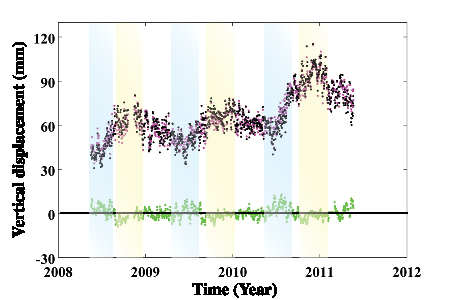
\includegraphics{figs_chpt3/2012GC004432-pA01.pdf}
	\caption[GPS time series from site SENU before (pink) and after (black) atmospheric pressure loading correction.]{GPS time series from site SENU before (pink) and after (black) atmospheric pressure loading correction. Green dots are vertical displacement due to atmospheric pressure loading. Light blue vertical bands mark approximate time period when atmospheric loading displacement is mainly positive. Light yellow vertical bands mark corresponding negative displacement.}
	\label{fig:SI3_fig1}
\end{figure}

\clearpage
\begin{figure}
	\centering
	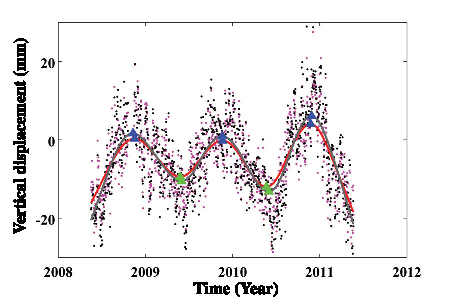
\includegraphics{figs_chpt3/2012GC004432-pA02.pdf}
	\caption[Example GPS time series for site SENU, de-trended and fit with annual model shown in Figure \ref{fig:fig2}.]{Example GPS time series for site SENU, de-trended and fit with annual model shown in \ref{fig:fig2}. Pink and black dots represent daily vertical position estimates before and after atmospheric pressure loading correction respectively. Red and grey curves are respective best-fit cubic splines with smoothing parameter set to 0.91.}
	\label{fig:SI3_fig2}
\end{figure}

\clearpage
\begin{figure}
	\centering
	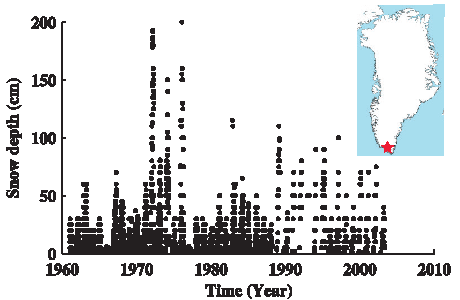
\includegraphics{figs_chpt3/2012GC004432-pA03.pdf}
	\caption[Snow depth recorded at a meteorological station  (WMO-ID 04272, Table \ref{tab:SI_chpt3_table2}) in southern Greenland coastal area.]{Snow depth recorded at a meteorological station  (WMO-ID 04272, Table \ref{tab:SI_chpt3_table2}) in southern Greenland coastal area.  Red star indicates location of the meteorological station.}
	\label{fig:SI3_fig3}
\end{figure}

\clearpage
\begin{figure}
	\centering
	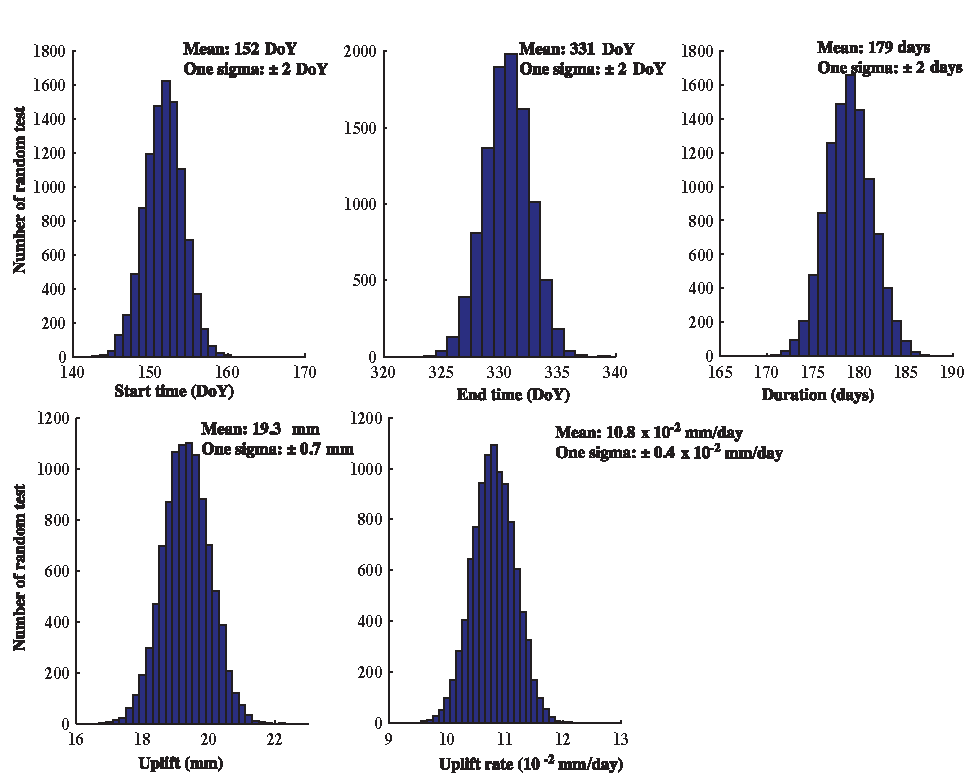
\includegraphics{figs_chpt3/2012GC004432-pA04.pdf}
	\caption[Histogram showing statistical result for five seasonal uplift variables at GPS station SENU.]{Histogram showing statistical result for five seasonal uplift variables at GPS station SENU.  Five variables are normally distributed.}
	\label{fig:SI3_fig4}
\end{figure}

\clearpage
\begin{figure}
	\centering
	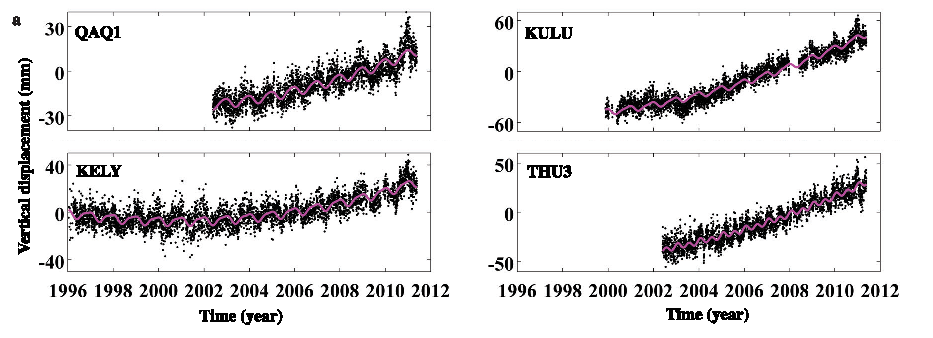
\includegraphics{figs_chpt3/2012GC004432-pA05a.pdf}
	\label{fig:SI3_fig5a}
\end{figure}

\clearpage
\begin{figure}
	\centering
	\includegraphics{figs_chpt3/2012GC004432-pA05b.pdf}
	\caption[Time series of GPS vertical component position.]{Time series of GPS vertical component position.  (a) Time series of long-term GPS records. (b) Time series of short-term GPS records.  For comparison with other sites, time series between mid-2007 and early 2011 at sites KULU, QAQ1, KELY and KULU are also shown in (b).  Vertical position is relative to arbitrary position. Pink curve shows constant acceleration model, including annual and semi-annual components.  GPS stations are organized from south to north.}
	\label{fig:SI3_fig5b}
\end{figure}

\clearpage
\begin{figure}
	\centering
	\includegraphics{figs_chpt3/2012GC004432-pA06a.pdf}
	\label{fig:SI3_fig6a}
\end{figure}

\clearpage
\begin{figure}
	\centering
	\includegraphics{figs_chpt3/2012GC004432-pA06b.pdf}
	\caption[Time series of GPS vertical component position after removing long-term trend by low pass filter.]{Time series of GPS vertical component position after removing long-term trend by low pass filter. (a) Time series of long-term GPS records. (b) Time series of short-term GPS records. In (b), we zoom in to the last 3 years of four long time series. Red curve is cubic spline best-fit model with 0.91 as smoothing parameter.  Blue triangle is the maximum value per year, and green triangle is the minimum value per year.}
	\label{fig:SI3_fig6b}
\end{figure}

\clearpage
\begin{figure}
	\centering
	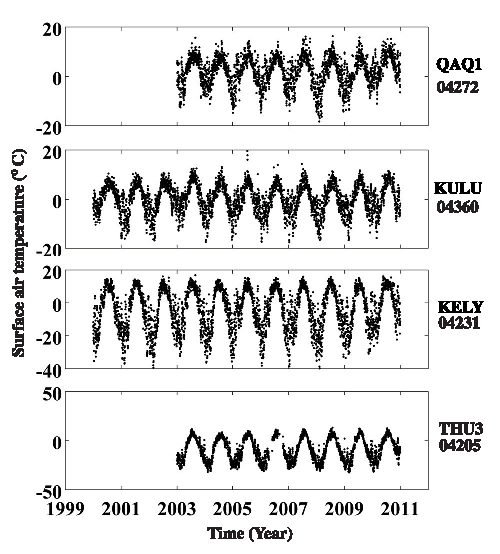
\includegraphics{figs_chpt3/2012GC004432-pA07.pdf}
	\caption[Time series of surface air temperature at meteorological stations near 4 GPS site.]{Time series of surface air temperature at meteorological stations near 4 GPS site.  Name of nearby GPS site and WMO-ID are on the right side of each plot. }
	\label{fig:SI3_fig7}
\end{figure}

%insert figures for chapter 4
\clearpage
\begin{figure}
\centering
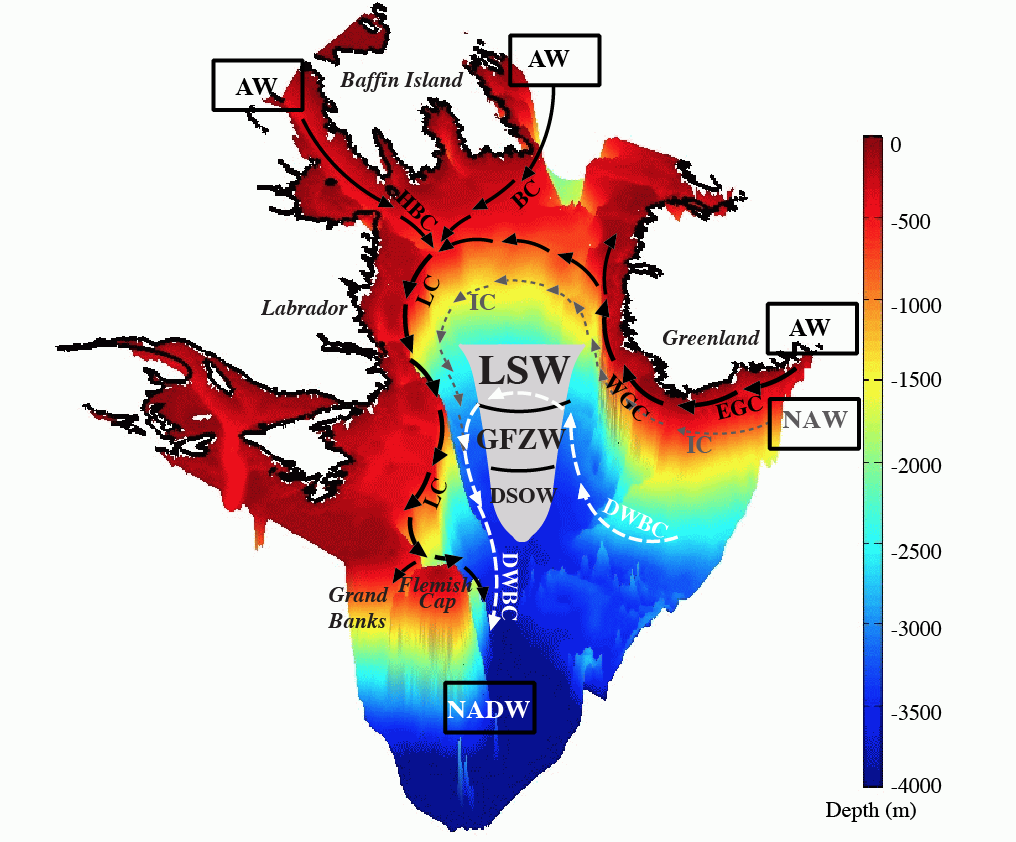
\includegraphics{figs_app/FigS1.png}
\caption[Simplified sketch illustrating 3-D structure of the Labrador Sea and major currents and water masses.]{Simplified sketch illustrating 3-D structure of the Labrador Sea and major currents and water masses. Black boxes represent water masses input to and output from the Labrador Sea along specific currents.  Arrows represent ocean currents at different depths: black solid arrows represent surface ocean currents carrying cold and fresh Arctic Water; grey dashed arrows represent subsurface ocean current carrying warm and salty North Atlantic Water; white dashed arrows represent the Deep Western Boundary Current that moves North Atlantic Deep Water southward.  EGC is East Greenland Current, WGC is West Greenland Current, HBC is Hudson's Bay Current, BC is Baffin Current, LC is Labrador Current, IC is Irminger Current, DWBC is Deep Western Boundary Current. AW is Arctic Water, NAW is North Atlantic Water, LSW is Labrador Sea Water, GFZW is Gibbs Fracture Zone Water, DSOW is Denmark Strait Overflow Water, NADW is North Atlantic Deep Water.  Not shown are the geographic sources of Arctic Water, which include the Greenland ice sheet, Arctic Ocean, Canadian Arctic Archipelago, and Hudson Bay, or the types of ice and water masses that contribute, which include glaciers and ice sheets, rivers, sea ice, and precipitation.  Also not shown are the major time scales for significant variability, which include annual (summer ice melting, winter cooling and convection) and decadal to multi-decadal (e.g., North Atlantic Oscillation, Atlantic Multi-decadal Oscillation).}
\label{fig:SI4_fig1}
\end{figure}

\begin{figure}
	\centering
	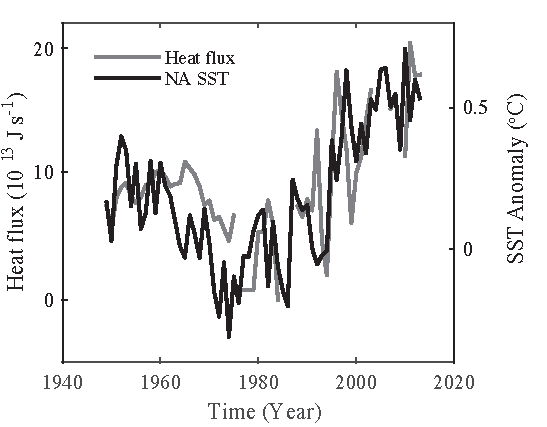
\includegraphics{figs_app/FigS2.pdf}
	\caption[Comparison of Irminger Water heat flux and North Atlantic SST anomaly over the period 1949 – 2013]{Comparison of Irminger Water heat flux and North Atlantic SST anomaly over the period 1949 – 2013.  Grey line indicates Irminger Water heat flux, black line indicates North Atlantic SST anomaly.  We use the HADISST dataset to compute SST anomaly.  We compute the annual average SST anomaly over a broad area of the North Atlantic, using as boundaries 0 $\textordmasculine$ - 60 $\textordmasculine$ North latitude and 0 $\textordmasculine$ - 80 $\textordmasculine$ West longitude, relative to the average temperature for the period 1901 to 1970.  Average North Atlantic SST anomaly shows a strong ($R=0.68$) and significant ($P=0.001$) correlation with our Irminger heat flux data for the 1949 to 2013 period, with both indices increasing strongly after 1995.}
	\label{fig:SI4_fig2}
\end{figure}

\begin{figure}
	\centering
	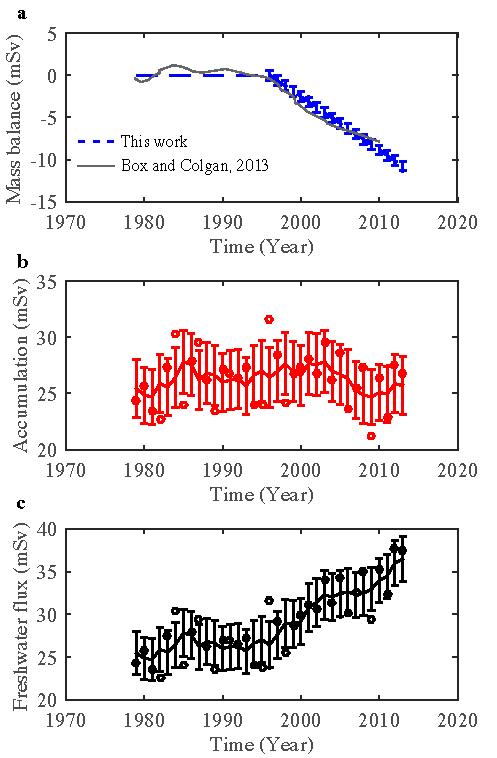
\includegraphics{figs_app/FigS3.pdf}
	\caption[Freshwater flux from Greenland estimated from mass balance and accumulation.  (a) Greenland mass balance.]{Freshwater flux from Greenland estimated from mass balance and accumulation.  (a) Greenland mass balance. Estimate from this study (blue dashed line) is compared with estimate from \citet{box2013greenland}. Blue error bars indicate uncertainty of mass balance, estimated at 95\% confidence level. (b) Greenland accumulation.  Red circles represent annual value.  Red solid line represents 5-year running average.  Red error bars indicate uncertainty of smoothed accumulation, which is approximated by uncertainty of accumulation modeled by RACMO2.3 ($\pm$ 9\%).  (c) Freshwater flux from Greenland.  Black circles represent freshwater flux from mass balance and annual accumulation (see equation \ref{eq:SI_chpt4_1}).  Black solid line represents freshwater flux from mass balance and smoothed accumulation.  Black error bars indicate propagated uncertainty.}
	\label{fig:SI4_fig3}
\end{figure}

\begin{figure}
	\centering
	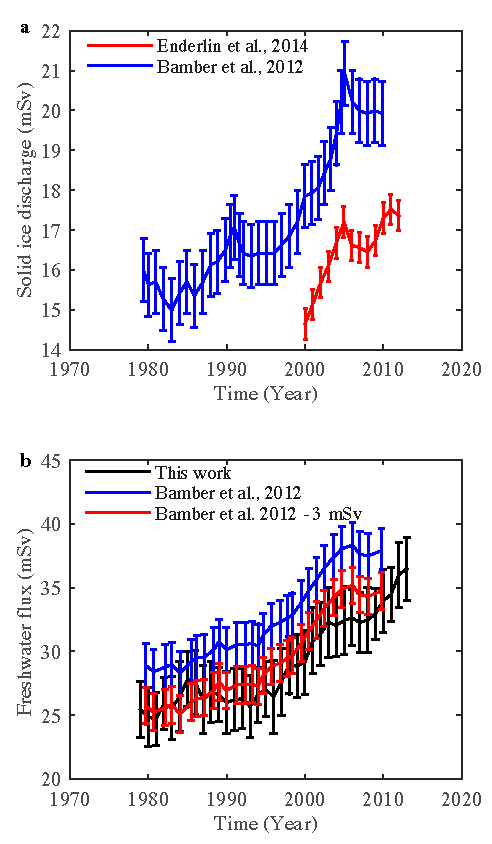
\includegraphics{figs_app/FigS4.pdf}
	\caption[Comparison between estimates of freshwater flux from Greenland.]{Comparison between estimates of freshwater flux from Greenland.  (a) Comparison between two estimates of solid ice discharge from Greenland.  Blue line from \citet{bamber2012recent}, red line from \citet{enderlin2014improved}.  The estimate from \citet{bamber2012recent} required extrapolation to cover all Greenland discharge and is $\sim$3 mSv ($\sim$100 km 3 yr$^{-1}$) larger than the more recent estimate from \citet{enderlin2014improved}. (b) Comparison of three estimates of freshwater flux from Greenland: black line (this study), blue line (\citet{bamber2012recent}), red line (\citet{bamber2012recent}) with correction following \citet{enderlin2014improved}.}
	\label{fig:SI4_fig4}
\end{figure}

\begin{figure}
	\centering
	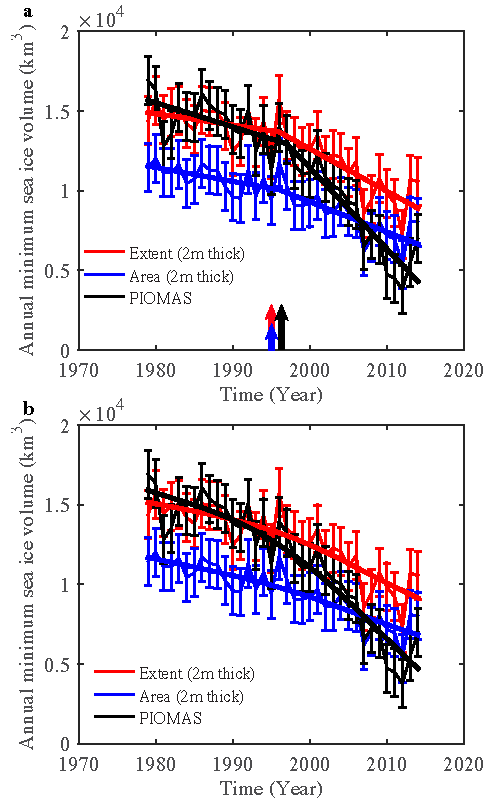
\includegraphics{figs_app/FigS5.pdf}
	\caption[Three estimates of the annual minimum Arctic sea ice volume time series.]{Three estimates of the annual minimum Arctic sea ice volume time series.  Red line represents estimate based on ice extent assuming 2 m thickness.  Blue line represents estimate based on ice area assuming 2 m thickness. Black line represents volume modeled by the Pan-Arctic Ice Ocean Modeling and Assimilation System (PIOMAS)\cite[]{zhang2003modeling}.  Error bars represent the uncertainty of annual minimum Arctic sea ice volume (1500 km$^{3}$).  (a) Three time series described above are fit with a two-slope model (thick solid line) (Supplementary methods).  Arrow marks the onset time of accelerated melting derived from three data sets: 1996 for ice extent and ice area data sets, 1997 for PIOMAS data set. (b) Three time series are fit with the linear state space model (thick solid line) (see methods in Appendix A). }
	\label{fig:SI4_fig5}
\end{figure}

\begin{figure}
	\centering
	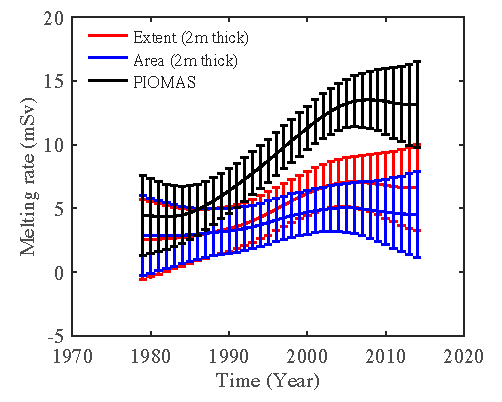
\includegraphics{figs_app/FigS6.pdf}
	\caption[Long term melting rate of Arctic sea ice from three data sets.]{Long term melting rate of Arctic sea ice from three data sets.  Red line represents estimate based on ice extent data set.  Blue line represents estimate based on ice area data set. Black line represents estimate from the Pan-Arctic Ice Ocean Modeling and Assimilation System (PIOMAS) data set. The melting rate is estimated using the linear state space model (Figure \ref{fig:SI4_fig5}b).  Error bars indicate uncertainty at 95\% confidence level.}
	\label{fig:SI4_fig6}
\end{figure}

\begin{figure}
	\centering
	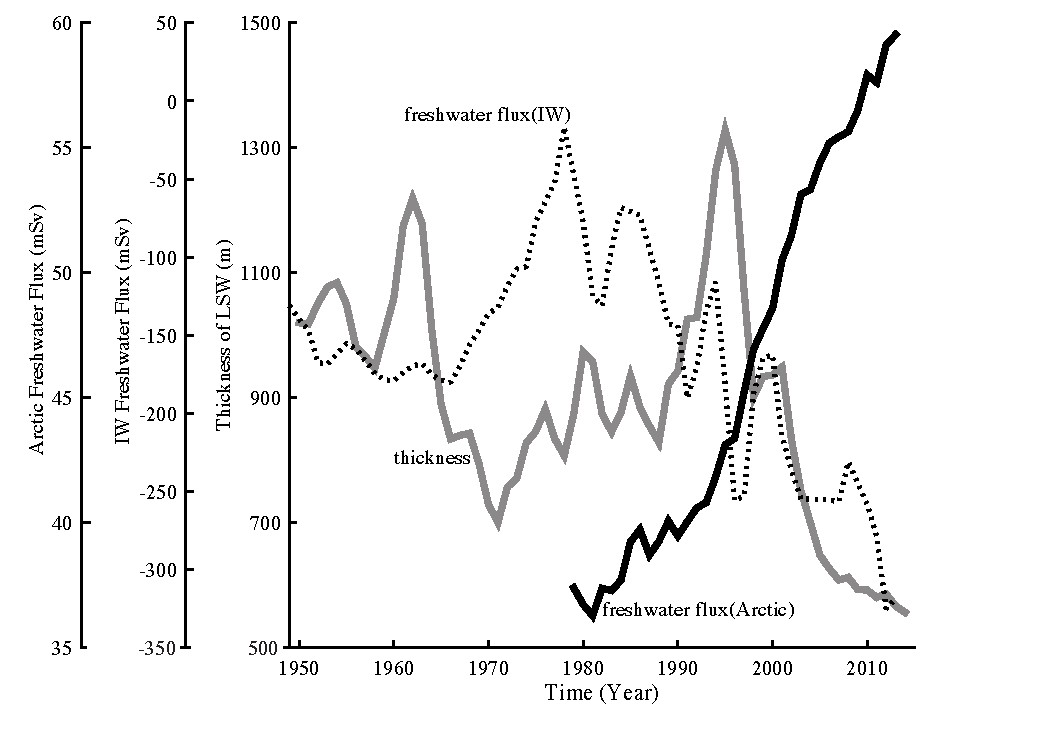
\includegraphics{figs_app/FigS7.pdf}
	\caption[Similar to Figure \ref{fig:chpt4_fig5} except salt flux of Irminger Water is expressed in terms of freshwater flux.]{Similar to Figure \ref{fig:chpt4_fig5} except salt flux of Irminger Water is expressed in terms of freshwater flux.  Grey solid line represents thickness of Labrador Sea Water.  Black solid line represents Arctic freshwater flux (the sum of freshwater flux from Greenland, the Canadian Arctic Archipelago and Arctic sea ice).  Dotted line represents freshwater flux of Irminger Water (IW). Salt flux is converted to freshwater flux using 34.80 as a reference salinity.}
	\label{fig:SI4_fig7}
\end{figure}

\begin{figure}
	\centering
	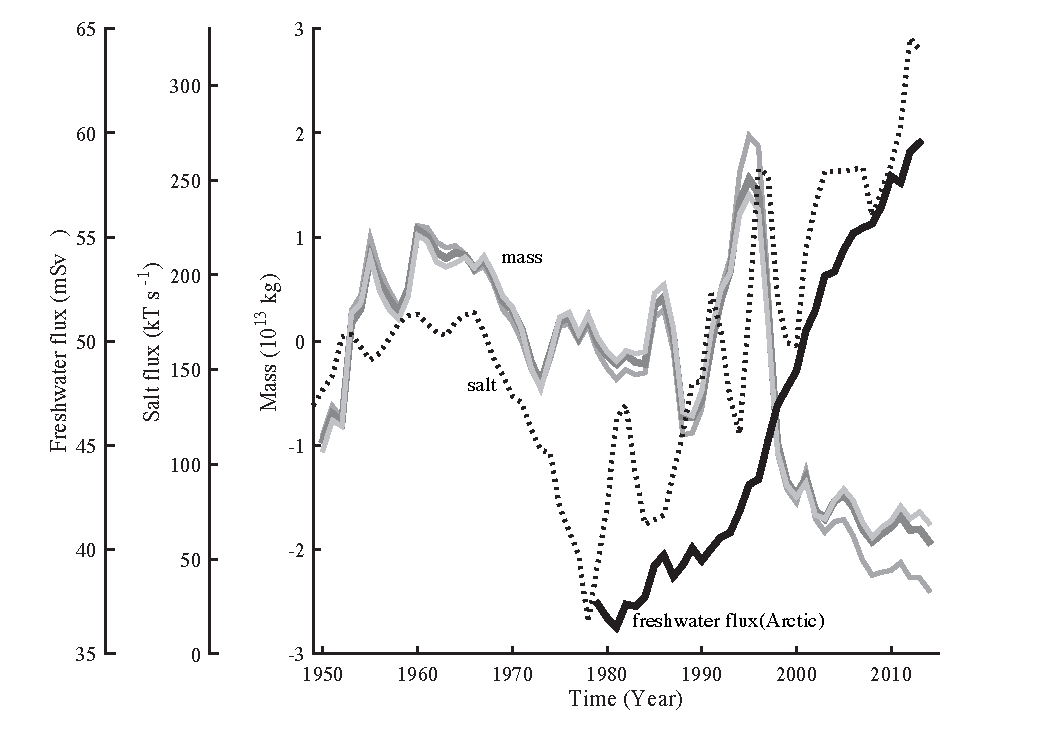
\includegraphics{figs_app/FigS8.pdf}
	\caption[Similar to Figure \ref{fig:chpt4_fig5} except grey solid line represents the mass of Labrador Sea Water.]{Similar to Figure \ref{fig:chpt4_fig5} except grey solid line represents the mass of Labrador Sea Water.  Black solid line represents Arctic freshwater flux (the sum of freshwater flux from Greenland, the Canadian Arctic Archipelago and Arctic sea ice). Density of Labrador Sea Water is obtained from the objective analyses of EN4.0.2 dataset from the UK Met Office Hadley Center\cite[]{good2013en4}.  Mass values are calculated by integrating density with volume between 50 $\textordmasculine$ N – 65 $\textordmasculine$ N, 38 $\textordmasculine$ W – 65 $\textordmasculine$ W and three depth range (900 – 2400 m, 1000 - 2500 m and 1100 – 2600 m), relative to the mean of 1950 – 2006. }
	\label{fig:SI4_fig8}
\end{figure}

\begin{figure}
	\centering
	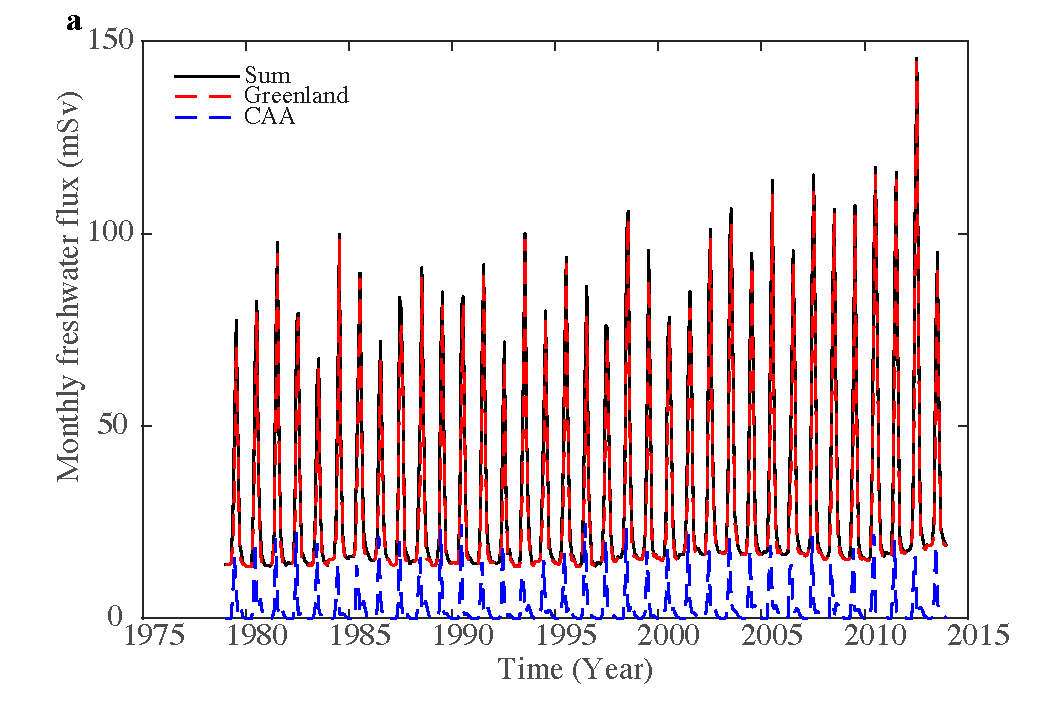
\includegraphics{figs_app/FigS9a.pdf}
\end{figure}

\begin{figure}
	\centering
	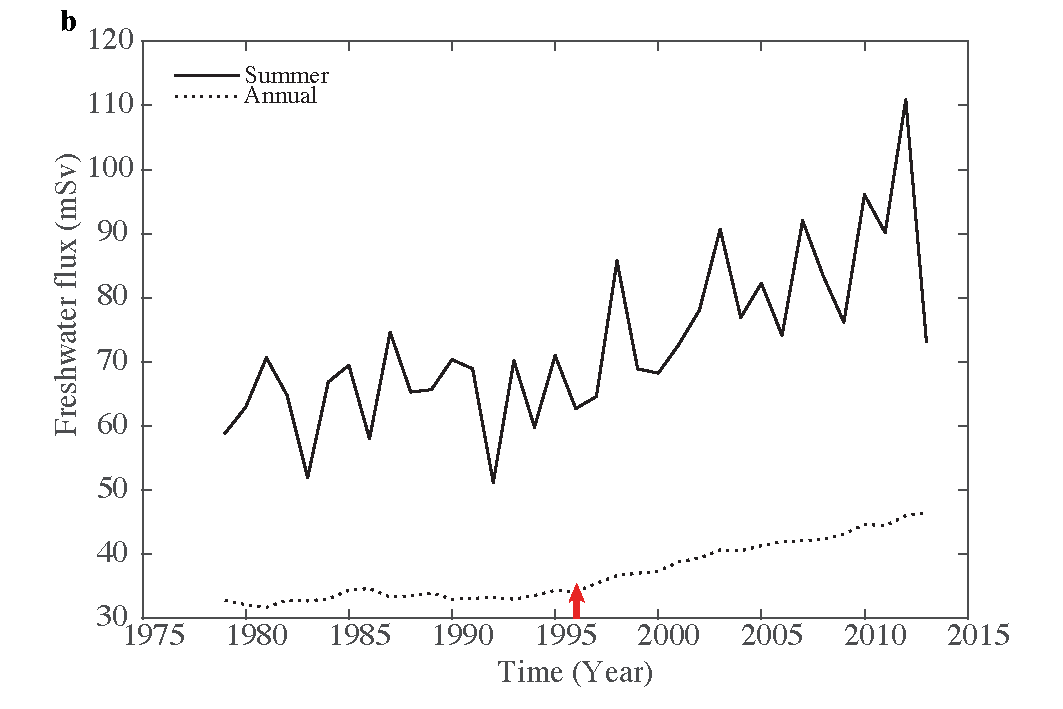
\includegraphics{figs_app/FigS9b.pdf}
	\caption[Seasonal variation of freshwater flux from Greenland and the Canadian Arctic Archipelago.]{Seasonal variation of freshwater flux from Greenland and the Canadian Arctic Archipelago. (a) Monthly freshwater flux from Greenland (GL), Canadian Arctic Archipelago (CAA) and their total for 1979 – 2013.   Freshwater flux from Greenland and CAA peaks in July.  Freshwater flux since 2002 has exceeded 100 mSv for about a month a year 9 times, with 2012 having the highest value (150 mSv).  (b) Total summer (June, July and August) freshwater flux (solid line) compared to long-term averaged annual freshwater flux (dashed line).  Note that summer freshwater flux increased significantly about the time when GRACE data and a simple model of constant acceleration suggest that the current phase of accelerated Greenland mass loss began (red arrow) (see Figure \ref{fig:chpt4_fig2}).}
	\label{fig:SI4_fig9}
\end{figure}

\begin{figure}
	\centering
	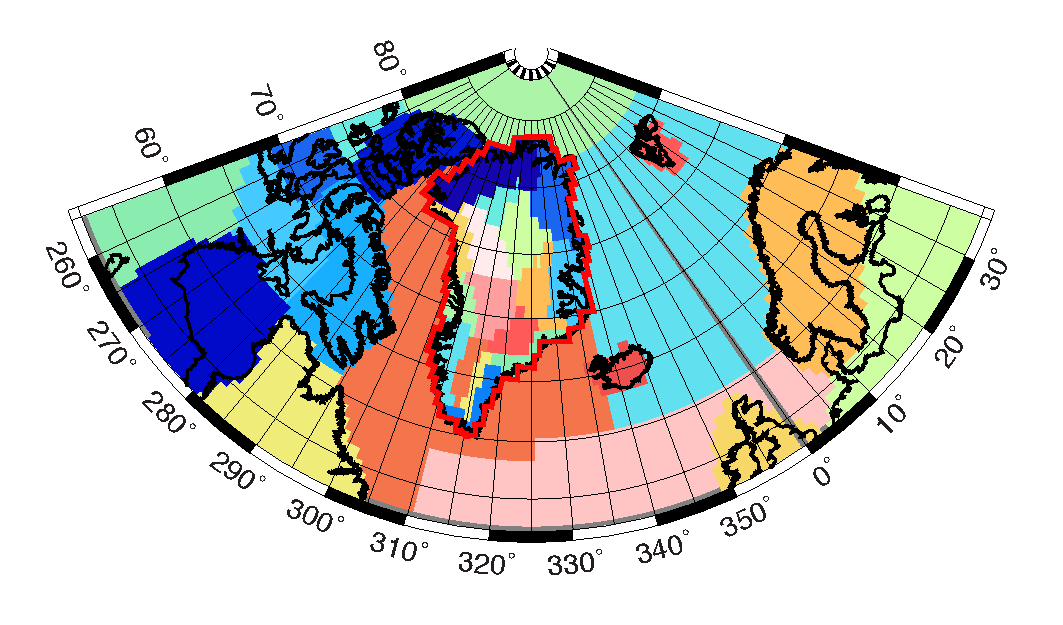
\includegraphics{figs_app/FigS10.pdf}
	\caption[Predefined regions used in this paper to localize the GRACE mass change signal.]{Predefined regions used in this paper to localize the GRACE mass change signal.  Greenland is outlined with solid red line.}
	\label{fig:SI4_fig10}
\end{figure}

\begin{figure}
	\centering
	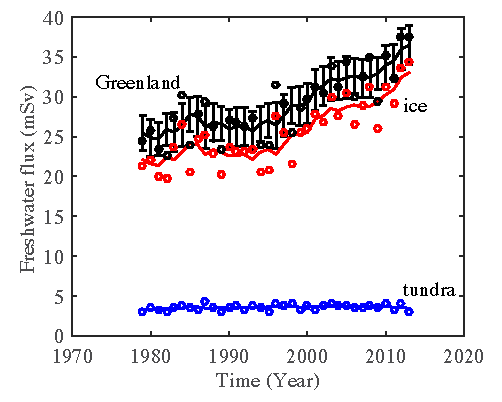
\includegraphics{figs_app/FigS11.pdf}
	\caption[Freshwater flux from Greenland and its two components.]{Freshwater flux from Greenland and its two components.  Black circles and solid line represent freshwater flux from Greenland.  Red circles and solid line represent freshwater flux component from ice mass loss.  Blue circles and solid line represent freshwater flux component from tundra runoff.  Circles represent annual value and solid line represents 5-year running average.  Black error bars indicate propagated uncertainty (Figure \ref{fig:SI4_fig3}).}
	\label{fig:SI4_fig11}
\end{figure}

\begin{figure}
	\centering
	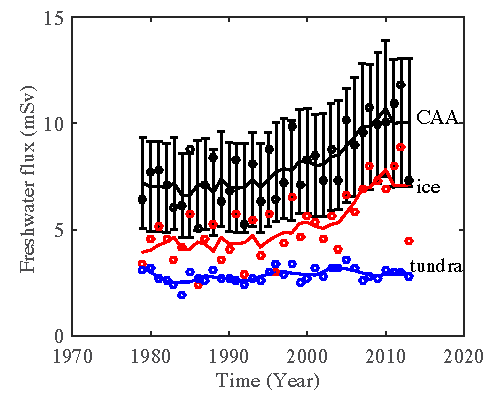
\includegraphics{figs_app/FigS12.pdf}
	\caption[Freshwater flux from the Canadian Arctic Archipelago and its two components.]{Freshwater flux from the Canadian Arctic Archipelago and its two components.  Black circles and solid line represent freshwater flux from the Canadian Arctic Archipelago (CAA).  Red circles and solid line represent freshwater flux component from ice mass loss.  Blue circles and solid line represent freshwater flux component from tundra runoff.  Circle represents annual value and solid line represents 5-year running average.  Black error bars indicate uncertainty of smoothed freshwater flux from CAA, approximated by uncertainty of runoff modeled by RACMO2.3, believed to be accurate to $\pm$ 30\%\cite[]{lenaerts2013irreversible}.}
	\label{fig:SI4_fig12}
\end{figure}